\documentclass[12pt]{ociamthesis}  % default square logo 
%\documentclass[12pt,beltcrest]{ociamthesis} % use old belt crest logo
%\documentclass[12pt,shieldcrest]{ociamthesis} % use older shield crest logo

%load any additional packages
\usepackage{amssymb}
\usepackage{multirow}
\usepackage{caption}
\usepackage{titlesec}
\usepackage{charter}
\usepackage{subfiles}
\usepackage{etoolbox} %halaman I-1
%\patchcmd{\addcontentsline}
 % {\thepage}
  %{\thechapter-\thepage}
  %{}
  %{}

\makeatletter
\@addtoreset{subsubsection}{chapter}
\makeatother
\renewcommand{\thepage}{\thechapter-\number\numexpr\arabic{page}\relax}
\patchcmd{\cleardoublepage}{\ifodd}{\unless\ifodd}{}{}
\preto\chapter{\cleardoublepage}
\AtBeginDocument{\setcounter{page}{1}}





\makeatletter					%
\renewcommand*\@pnumwidth{3em}	% ratain halaman daftar isi
\makeatother					%

\title{\large    %your thesis title,
        Pemrograman II}   %note \\[1ex] is a line break in the title
        

\author{Diajukan untuk memenuhi kelulusan matakuliah Pemrograman II Program Studi DIV Teknik Informatika\\[5ex]
O l e h : \\
[1ex] Naomi C.H Tampubolon   \\ 
\textbf{1.18.4.018}\\
		 [5ex] } 
		 
\college{}  %your college

%\renewcommand{\submitt edtext}{change the default text here if needed}
\degree{POLITEKNIK POS INDONESIA}    %the degree
\degreedate{\textbf{BANDUNG\\2019}}  

%end the preamble and start the document
\begin{document}

%this baselineskip gives sufficient line spacing for an examiner to easily
%markup the thesis with comments
\baselineskip=18pt plus1pt

%set the number of sectioning levels that get number and appear in the contents
\setcounter{secnumdepth}{3}
\setcounter{tocdepth}{3}


\maketitle          % create a title page from the preamble info

\begin{romanpages}


          % start roman page numbering
\addcontentsline{toc}{chapter}{DAFTAR ISI}
\tableofcontents            % generate and include a table of contents
\addcontentsline{toc}{chapter}{DAFTAR GAMBAR}

\end{romanpages}   
\chapter*{Teori}

\begin{enumerate}
	\item CSV(Comma Separated Value) adalah format data yang digunakan para pengguna untuk menginputkan data kedalam database secara sederhana.

	\begin{itemize}
	\item Fungsi file CSV adalah format basis data sederhana yang di setiap record dipisahkan dengan tanda koma dan titik koma.
	\end{itemize}
	
	\begin{figure} [h]
	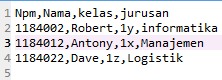
\includegraphics[width=5cm]{poto/1.png}
	\centering
	\end{figure}		
	
	
	
	
	\item Aplikasi yang dapat membuat file CSV adalah Notepad,Worpad,Microsoft Excel,dll
	
	\item Cara membuat file CSV:
	\begin{itemize}
	\item Buka Ms.Excell
	\end{itemize}
	\begin{itemize}
	\item Membuat data di Ms.Excel
	\end{itemize}
	\begin{itemize}
	\item Lalu pada saat menyimpan pilih "save as" dan jenis file nya diganti csv
	\end{itemize}
	\begin{itemize}
	\item Dan file CSV telah dibuat
	\end{itemize}

	\item library csv adalah format yang sudah digunakan selama bertahun-tahun dengan cara standar di RFC 4180. Perbedaan halus terdapat di beberapa aplikasi.
	
	
	\item library Pandas adalah alat analisis data dan struktur unruk bahasa pemrograman Python.  Panda digunakan dengan mudah untuk mengelola data salah satu fiturnya adalah Dataframe. Dataframe dapat digunakan untuk membaca sebuah file dan menjadikannya table.


	\item Fungsi yang terdapat pada library CSV:\\
	\begin{itemize}
	\item Reade, Fungsi Reader diguunakan untuk membaca  isi file
	\end{itemize}
	\begin{itemize}
	\item Dict Reader, Fungsi Dict Reader digunakan untuk membaca isi file yang terdapat di dictionary
	\end{itemize}
	\begin{itemize}
	\item Write, Fungsi Write ini digunakan untuk menulis file
	\end{itemize}
	\begin{itemize}
	\item Dict Write, Fungsi Dict Write digunakan untuk menulis file yang ada di dictionary
	\end{itemize}
	
	\item Fungsi yang terdapat di libarary pandas
	\begin{itemize}
	\item to\_csv, untuk menulis file yang type nya CSV
	\end{itemize}
	\begin{itemize}
	\item read\_csv, untuk membaca file type CSV
	\end{itemize}
	
	
\end{enumerate}



\chapter{Ketrampilan Pemrograman}

\section{Nomor 1}
\lstinputlisting[language=Python, firstline=4, lastline=8]{src/1184047_realtime.py}
\section{Nomor 2}
\lstinputlisting[language=Python, firstline=3, lastline=8]{src/1184047_save.py}
\section{Nomor 3}
\lstinputlisting[language=Python, firstline=10, lastline=18]{src/1184047_realtime.py}
\section{Nomor 4}
\lstinputlisting[language=Python, firstline=4, lastline=16]{src/1184047_csv.py}
\chapter{Laporan}
\section{PEMAHAMAN TEORI}
\subsection{FUNGSI}
\begin{enumerate}
	\item Fungsi adalah salah satu blok program yang sudah terorganisir terdiri dari nama fungsi, input variabel dan variabel kembalian. Fungsi digunakan untuk aplikasi anda dan tingkat penggunaan kode yang tinggi agar aplikasi lebih baik.
	\item inputan fungsi digunakan untuk menerima baris input dari user dan mengembalikannya dalam bentuk string.
	\item kembalian fungsi yaitu fungsi akan membaca sebaris input umumnya melalui keyboard sampai nanti dijumpai karakter newline(enter) dan akan mengembalikan string dari inputan tersebut.  
\end{enumerate}
\lstinputlisting[language=Python]{src/KodingTeori1.py}

\subsection{PAKET}
\begin{enumerate}
\item Paket adalah sebuah manifestasi dari konsep namespace hierarkis python.
\item cara pemanggilan paket  
\lstinputlisting[language=Python]{src/KodingTeori2.py}
\end{enumerate}

\subsection{KELAS}
\begin{enumerate}
\item kelas adalah prototipe yang ditentukan oleh pengguna untuk objek yang mendefinisikan seperangkat atribut yang menjadi ciri khas dari sebuah kelas apa pun. Class digunakan untuk membuat kelas baru dan nama kelas diikuti kanca kunci titik dua. 
\item Objek adalah perwujudan dari sebuah class. Bila kelas adalah prototipe nya, dan objek adalah barang jadinya. 
\item atribut yaitu semua class yang membuat objek dan semua objek tersebut mengandung karakteristik.
\item method merupakan fungsi yang didefinisikan di dalam suatu class.
\end{enumerate}
\lstinputlisting[language=Python]{src/KodingTeori3.py}
\subsection{Cara pemanggilan library kelas dari instansiasi dan pemakaiannya contoh dengan program}
untuk membuat objek dari sebuah kelas, kita memanggil nama kelas dengan argumen yang sesuai dengan   fungs pada saat kita mendefinisikannya.
\\cara pemanggilan\\
\lstinputlisting[language=Python]{src/KodingTeori4.py}
\subsection{Pemakaian paket dengan perintah from kalkulator import penambahan}
Pertama-tama kalian harus membuat program kalkulator.py untuk bisa melakukan penambahan sperti di bawah
\lstinputlisting[language=Python]{src/KodingTeori5.py}
\subsection{Pemakaian paket fungsi apabila file library ada di dalam folder}
Untuk pemakaian paket fungsi apabila file library berada di folder yaitu untuk dapat melakukan atau menjalankan kalkulator yang berada di file folder.
\lstinputlisting[language=Python]{src/KodingTeori6.py}
\subsection{Pemakaian paket kelas apabila file library ada di dalam folder}
Untuk pemakaian paket kelas apabila file library berada di folder.Mahasiswa yaitu file Mahasiswa untuk melakukan atau menjalankan kode yang berada di file folder Mahasiswa tersebut.
\lstinputlisting[language=Python]{src/KodingTeori7.py}
\section{KETERAMPILAN PEMROGAMAN}
\lstinputlisting[language=Python]{src/NPM1.py}
\lstinputlisting[language=Python]{src/NPM2.py}
\lstinputlisting[language=Python]{src/NPM3.py}
\lstinputlisting[language=Python]{src/NPM4.py}
\lstinputlisting[language=Python]{src/NPM5.py}
\lstinputlisting[language=Python]{src/NPM6.py}
\lstinputlisting[language=Python]{src/NPM7.py}
\lstinputlisting[language=Python]{src/NPM8.py}
\lstinputlisting[language=Python]{src/NPM9.py}
\lstinputlisting[language=Python]{src/NPM10.py}
\lstinputlisting[language=Python]{src/kalkulator.py}
\lstinputlisting[language=Python]{src/Mahasiswa.py}
\lstinputlisting[language=Python]{src/Ngitung.py}
\lstinputlisting[language=Python]{src/3lib.py}
\lstinputlisting[language=Python]{src/main.py}
\lstinputlisting[language=Python]{src/kelas3lib.py}
\lstinputlisting[language=Python]{src/main.py}
\section{KETERAMPILAN PENANGANAN ERROR}
\lstinputlisting[language=Python]{src/KeterampilanPenangananError.py}
\section{LAMPIRAN PLAGIARISM}
\begin{figure}[H]
		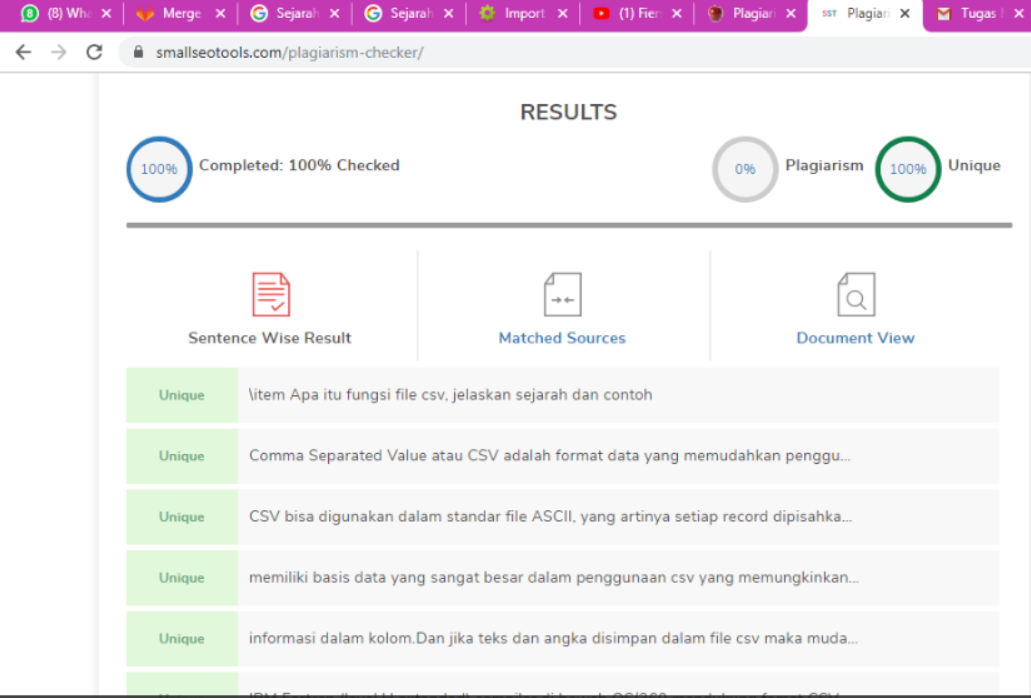
\includegraphics[width=4cm]{figures/1184065/ss1.PNG}
		\centering
		\caption{Screnshoot Plagiarism}
	\end{figure}
	\begin{figure}[H]
		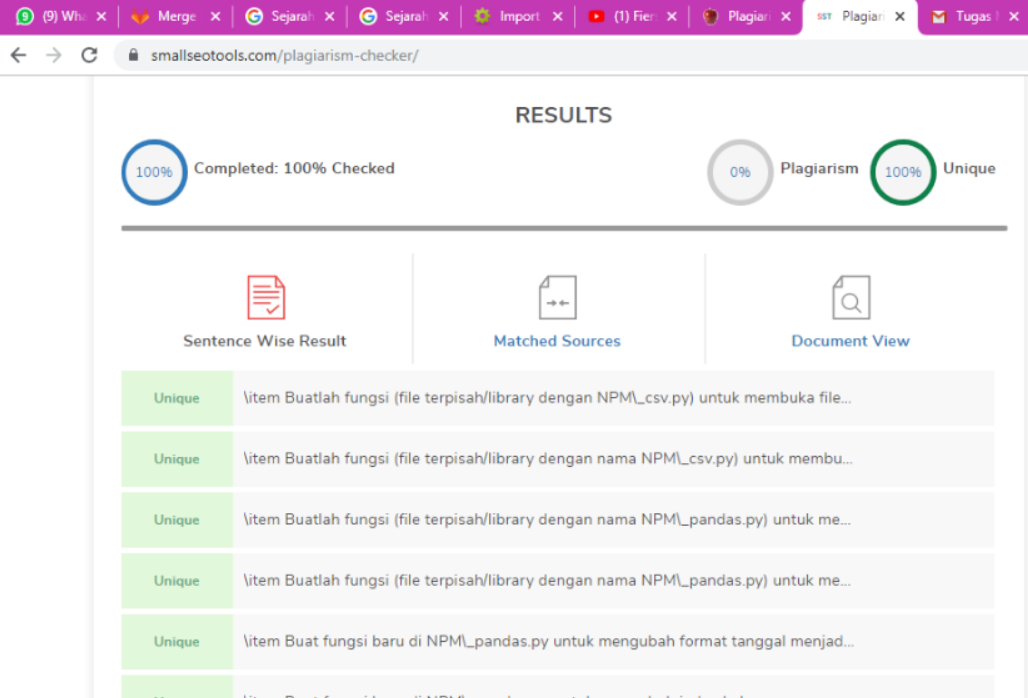
\includegraphics[width=4cm]{figures/1184065/ss2.PNG}
		\centering
		\caption{Screnshoot Plagiarism}
	\end{figure}
\section{LINK YOUTUBE}
\begin{enumerate}
\item \href{https://youtu.be/FDE8KrHC4m4}{klik}
\item \href{https://youtu.be/qzmEN1LVhsM}{klik}
\item \href{https://youtu.be/3UKVrJmwmYo}{klik}
\item \href{https://youtu.be/3UKVrJmwmYo}{klik}
\end{enumerate}








\chapter{Pengelolaan File CSV}

Tujuan pembelajaran pada pertemuan keempat antara lain:
\begin{enumerate}
\item
Mengenal file CSV dan fungsinya 
\item
Mengerti cara memakai library CSV
\item
Mengerti cara memakai library pandas
\item
Mengatasi Error yang terjadi akibat pemakaian library csv dan pandas
\item
Try Except
\end{enumerate}
Tugas dengan cara dikumpulkan dengan pull request ke github dengan menggunakan latex pada repo yang dibuat oleh asisten IRC. Kode program dipisah dalam folder src NPM.py yang berisi praktek dari masing-masing tugas file terpisah sesuai nomor yang kemudian dipanggil menggunakan input listing ke dalam file latex penjelasan atau nomor pengerjaan. Masing masing soal bernilai 5 dengan total nilai 100. Gunakan bahasa yang baku dan bebas plagiat dengan dibuktikan hasil scan plagiarisme. Serta hasil scrinsut dari komputer sendiri, dan kode hasil sendiri. Pengerjaan menggunakan latex dan harus menyertakan file pdf hasil compile pdflatex, jika tidak diskon 50\%.


\section{Pemahaman Teori}
Kerjakan soal berikut ini, masing masing bernilai 5. Untuk hari pertama.
Praktek teori penunjang yang dikerjakan dengan deadline besok jam 4 pagi:
\begin{enumerate}
\item
Apa itu fungsi file csv, jelaskan sejarah dan contoh
\item
Aplikasi-aplikasi apa saja yang bisa menciptakan file csv?
\item
Jelaskan bagaimana cara menulis dan membaca file csv di excel atau spreadsheet
\item
Jelaskan sejarah library csv
\item
Jelaskan sejarah library pandas
\item
Jelaskan fungsi-fungsi yang terdapat di library csv
\item
Jelaskan fungsi-fungsi yang terdapat di library pandas
\end{enumerate}

\section{Ketrampilan Pemrograman}
Kerjakan soal berikut ini, masing masing bernilai 5 untuk hari kedua, lusa jam 4 pagi. Soalnya adalah:

\begin{enumerate}
\item
Buatlah fungsi (file terpisah/library dengan nama NPM\_csv.py) untuk membuka file csv dengan lib csv mode list
\item
Buatlah fungsi (file terpisah/library dengan nama NPM\_csv.py) untuk membuka file csv dengan lib csv mode dictionary
\item
Buatlah fungsi (file terpisah/library dengan nama NPM\_pandas.py) untuk membuka file csv dengan lib pandas mode list
\item
Buatlah fungsi (file terpisah/library dengan nama NPM\_pandas.py) untuk membuka file csv dengan lib pandas mode dictionary
\item
Buat fungsi baru di NPM\_pandas.py untuk mengubah format tanggal menjadi standar dataframe
\item
Buat fungsi baru di NPM\_pandas.py untuk mengubah index kolom
\item
Buat fungsi baru di NPM\_pandas.py untuk mengubah atribut atau nama kolom
\item
Buat program main.py yang menggunakan library NPM\_csv.py yang membuat dan membaca file csv
\item
Buat program main2.py yang menggunakan library NPM\_pandas.py yang membuat dan membaca file csv
\end{enumerate}




\section{Ketrampilan Penanganan Error}
Kerjakan soal berikut ini, masing masing bernilai 5(hari kedua). Bagian Penanganan error dari script python.
\begin{enumerate}
\item
Tuliskan peringatan error yang didapat dari mengerjakan praktek ketiga ini, dan jelaskan cara penanganan error tersebut.
dan Buatlah satu fungsi yang menggunakan gunakan try except untuk menanggulangi error tersebut.
\end{enumerate}



\section{Presentasi Tugas}
Pada pertemuan ini, diadakan dua penilaiain yaitu penilaian untuk tugas mingguan seperti sebelumnya dengan nilai maksimal 100. Kemudian dalam satu minggu kedepan maksimal sebelum waktu mata kuliah kecerdasan buatan. Ada presentasi kematerian dengan nilai presentasi yang terpisah masing-masing 100. Jadi ada tiga komponen penilaiain pada pertemuan ini yaitu :
\begin{enumerate}
	\item tugas minggu hari ini dan besok (maks 100). pada chapter ini
	\item presentasi csv (maks 100). Mempraktekkan kode python dan menjelaskan cara kerjanya.
\end{enumerate}
Waktu presentasi pada jam kerja di IRC. Kriteria penilaian presentasi sangat sederhana, presenter akan ditanyai 20(10 pertanyaan program, 10 pertanyaan teori) pertanyaan tentang pemahamannya menggunakan python untuk kecerdasan buatan. jika presenter tidak bisa menjawab satu pertanyaan asisten maka nilai nol. Jika semua pertanyaan bisa dijawab maka nilai 100. Presentasi bisa diulang apabila gagal, sampai bisa mendapatkan nilai 100 dalam waktu satu minggu kedepan.





\chapter{Link Youtube}

Link youtube : \textbf{\textit{https://youtu.be/bAWhfxgnPKE}}



%next line adds the Bibliography to the contents page
\addcontentsline{toc}{chapter}{Daftar Pustaka}
%uncomment next line to change bibliography name to references
%\renewcommand{\bibname}{References}
\bibliography{references}    %use a bibtex bibliography file refs.bib
\bibliographystyle{plain}  %use the plain bibliography style


\end{document}

